\section{Pipeline - Local configuration}
\label{sec:pipeline-local}
The localized pipeline is constructed with the components 
that are described in section \ref{sec:tools}, but the components are:

\begin{itemize}
    \item Gitea
    \item Drone
    \item Nginx
    \item Docker
    \item Local registry
    \item Certificate 
\end{itemize}
\subsection{Pipeline deployment}
\label{sec:pipeline-local-deployment}
The deployment of the pipeline is currently only available for certain operating systems. The operating systems that are supported are
\javaf{Ubuntu} and \javaf{Kali}. The deployment is done through a script \javaf{prerun.sh} that is located in the src directive of the repository.
The script consist of two parts. 
\paragraph{Part 1} of the script controls all the prerequisites that are needed for the pipeline to run. Without 
these prerequisites, the pipeline will not be able to run. The prerequisites are:
\begin{itemize}
    \item Package control. The script needs a certain number of specific packages to be installed. The packages are: \javaf{docker},
    \javaf{docker-compose}, \javaf{curl}, \javaf{python3}, \javaf{jq}, and \javaf{openssl}. There are also some packages needed that are not listed, 
    but they are preinstalled on all Ubuntu\cite{ubuntu} and Kali\cite{kali} systems.
    \item Creation of a \javaf{docker network}. This network is where all the containers will be located and communicate over.
    This network is also where the gateway to the reverse proxy is located. Without this network, the user would not be able to communicate with the pipeline.
    \item When the \javaf{docker network} is created, the script will insert a \ac{DNS} record in the 
    \javaf{/etc/hosts} file generic to Ubuntu and Kali systems. This is done so that the user can access the website with a \ac{DNS} record.
    \item Last in the first part of the script is the insertion of the certificate created for 
    the pipeline. The certificate needs to be inserted into the hosts\\
    \javaf{/etc/ssl/certs/ca-certificates.crt} file because the drone runners will use the host volumes for its certificate.
\end{itemize}
The first part of the script ensures that all prerequisites are met. The final command of part 1 initiates the spawning of containers. 
The script uses Docker Compose for this task, and the command used is shown in Figure \ref{fig:docker-compose-localized}.\\
When the first part is complete without error, the script shown in Figure \ref{fig:docker-compose-localized}.
\begin{figure}[h]
    \begin{center}
        \javaf{docker compose --env-file .env up --build -d}
    \end{center}
    \caption{docker compose command to spawn localized pipeline containers}
    \label{fig:docker-compose-localized}
\end{figure}


\paragraph{Second part} of the script waits for the containers to be up and running.
All the commands in the second part of the script is a health check to see if everything is running correctly.
It is also to make the user wait until everything works. Some of the containers depends on other containers, and 
therefore if interacted with before those containers are ready, would mean that there could be a potential error.


\subsection{Gitea}
\label{sec:pipeline-local-gitea}

When Gitea is running it must be fully configurated and ready to be interacted with.
This setup begins in the \javaf{Dockerfile.gitea}, 
where the Gitea instance is built with the necessary configurations. If Gitea does not receive an initial configuration, 
the user will encounter an initial setup page upon their first visit to Gitea, as shown in Figure \ref{fig:gitea-setup}.
\begin{figure}[h]
    \centering
    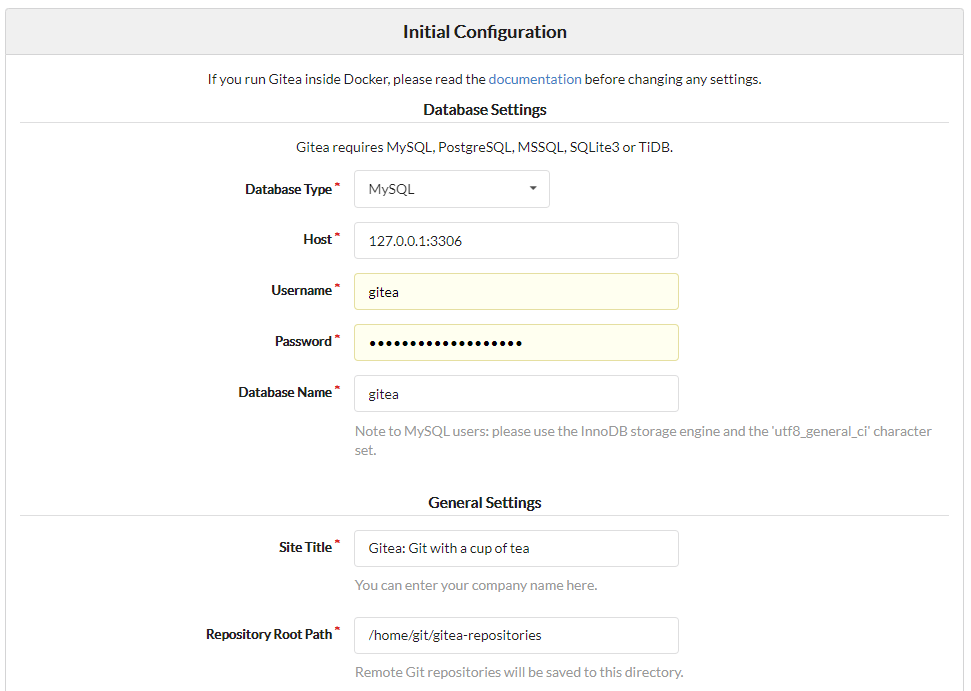
\includegraphics[width=0.8\textwidth]{images/initial_conf.png}
    \caption{Gitea setup page}
    \label{fig:gitea-setup}
\end{figure}
To avoid this, the deployment is provided with two things.

\textbf{First} is the \javaf{app.ini} file, which is the configuration file for Gitea. If no \javaf{app.ini} file is provided, 
it will be populated with data from the initial configuration page. The \javaf{app.ini} file is located in \javaf{src/gitea/config/app.ini}.

\textbf{Second} is a minimal installation of Gitea. This minimal installation is found in \javaf{src/gitea/config/gitea.tar.gz}. 
It is a simple setup of Gitea that, after the initial configuration, takes only a minute to set up. By placing the \javaf{gitea.tar.gz} file in the container 
directory \javaf{\data}, the Gitea instance will be set up with this minimal installation.
After initialization of Gitea, the script \javaf{src/gitea/start.sh} is run.
The script will curl the Gitea application to wait until Gitea is running.
The script will create \javaf{users}, \javaf{tokens}, \javaf{webhooks}, \javaf{Oauth} and \javaf{Oauth_grant}.
The script collects the information about these things from \javaf{src/gitea/config/}.

\subsection{Drone}
\label{sec:pipeline-local-drone}
Drone uses a script to initialize all the infrastructure supporting the pipeline and the underlying \ac{CTF}'s. 
Typically, when the drone is initialized, it contains no users or information about repositories. However, for a localized pipeline, 
it would be highly advantageous to have repositories and users present before the users first log in to the pipeline.

The initialization script for Drone resides in \javaf{src/drone/init.sh}. 
Since there is no direct access to the Drone data before the actual program starts through the 
\ac{API} or \ac{CLI}, a database.sql file is created, manipulated, and fed to the Drone container.
Drone utilizes a SQLite database, and data is inserted into the database using \javaf{sqlite3} commands. 
An example of a command used to insert users into the Drone database is depicted in Figure \ref{fig:sqlite3-insert}. 
The complete script can be viewed in the source code.

\begin{figure}
    \begin{center}
        \javaf{sqlite3 /data/database.sqlite "INSERT INTO users"}
    \end{center}
    \caption{sqlite3 command to insert users into the drone database}
    \label{fig:sqlite3-insert}
\end{figure}

To create and define these users and repositories before the drone program starts, 
they must match exactly on the Gitea side. 
Drone utilizes configuration files from the \javaf{src/drone/config/} 
folder to create the users and repositories. The configuration data in these \ac{CSV} files are identical to those used to create users and push repositories to Gitea.

\subsection{Nginx proxy}
\label{sec:pipeline-local-nginx}

Whenever a user interacts with the infrastructure, it will 
request by \ac{DNS} record to the gateway of the Docker Network, nginx reverse proxy, when then pickup that request, and 
proxy it to the correct container. The reverse proxy is also located inside a container, and is able through the Docker network,
to communicate with other containers. If another container outside the \javaf{docker network}
would like to communicate with a application inside the network, it would have to
go through the reverse proxy.

As described in section \ref{sec:nginx}, the reverse proxy is configuration is located in \javaf{src/proxy/default.conf}.
The conf file has three server blocks which includes the \javaf{ssl_certificate}, \javaf{ssl_conf}, and the \javaf{proxy_pass}.
These three things define what the reverse proxy does whenever a user calls the DNS record. The \ac{DNS} record for a 
specific server block is defined as \javaf{server_name}. The configuration for the proxy pass to Gitea is shown in Figure \ref{fig:nginx-proxy-pass}.

\begin{figure}[h]
    \centering
    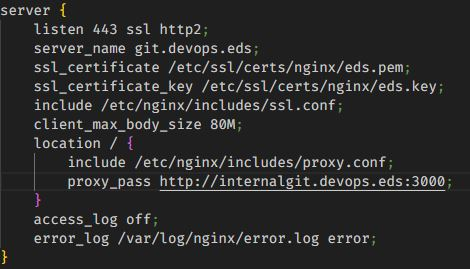
\includegraphics[scale=.7]{images/git_proxy_pass.jpg}
    \caption{Nginx proxy pass to Gitea}
    \label{fig:nginx-proxy-pass}
\end{figure}

\subsection{Docker}
\label{sec:pipeline-local-docker}
Docker serves as the backbone of the pipeline, facilitating easy deployment, maintenance, and development. 
Leveraging Docker as the containerization tool enables deployment and utilization across various environments. 
The Docker containers are specified in the \javaf{docker-compose.yml} file, located within the \javaf{src} directory.

Docker will spawn five containers and attach itself to the Docker network, when the \javaf{prerun} script is run.
\javaf{Nginx}, \javaf{Gitea}, \javaf{Drone}, \javaf{Registry}, and \javaf{Drone-runners}.
Whenever the pipeline is spawned Docker will create new images. This is to make sure that, if new changes are made 
that they are included in the new run. Docker can sometimes force itself to use cached images instead of building new 
ones if the changes are small.

The configuration for the pipeline all relies in the \javaf{docker-compose.yml} file. If any of the link, volumes, network etc. 
is wrongly configured, the pipeline might run, but it might mean that a CTF or a webhook will not create the desired outcome.\\
Differently from the remote pipeline, in the localized pipeline, Gitea and Drone are supplied with the Oauth2 application and Oauth2 grant
before it is initialized. 
By doing so, the user will not have to go through the initial setup of the application and will have access 
right away to Drone without having to authenticate through Gitea.

\subsection{Registry}
\label{sec:pipeline-local-registry}
As the project needed a local registry to fetch and push images into, the registry is a crucial part of the pipeline.
The registry used is developed by Distribution.\cite{registry}
The registry is a image registry similar to DockerHub, although DockerHub is actually isn't a registry, but a 
frontend to view available images. 
Typically, when users use the \javaf{docker pull} command, images are fetched from DockerHub. 
However, when utilizing a local registry, ensuring that images are pulled from it requires specific steps. 
The container hosting the registry must include a designated \javaf{certs} folder to inform Docker that the local registry, 
which employs a self-signed certificate, is a trusted source.\\
To establish trust in the untrusted registry mirror, the certificate must be placed in the root Docker configuration folder, specifically in \\ 
\javaf{/etc/docker/certs.d/}, with the URL of the registry, in this case, being \\
\javaf{registry.devops.eds}.
Then whenever a users or a runner wants to pull an image from the registry, it will have to use the specific URL.
see figure \ref{fig:specific_registry_url} for 
an example of a image pull in a pipeline.\\
\begin{figure}
    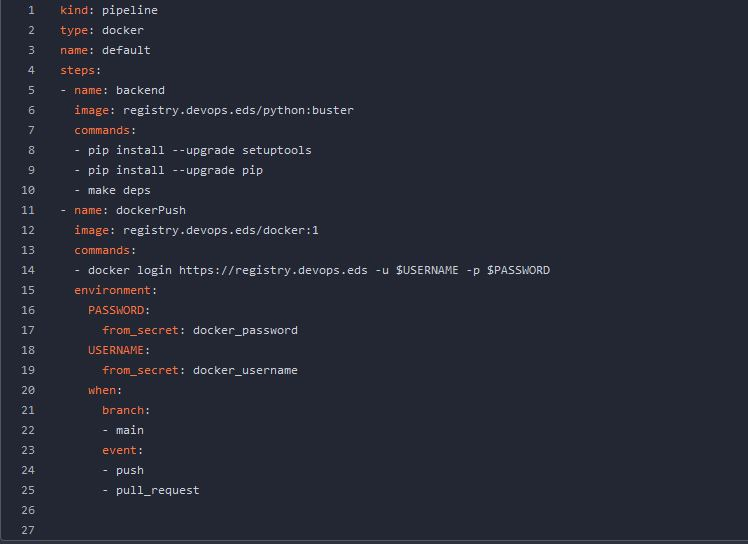
\includegraphics[scale=0.65]{images/local-registry-pull.jpg}
    \caption{Pulling an image from the local registry}
    \label{fig:specific_registry_url}
\end{figure}
The local registry work just like \url{https://registry-1.docker.io}. Although it different from \url{https://hub.docker.com}
. DockerHub is the a UI to find version and images, but isn't the actual registry where the images are stored.

\subsection{Certificate}
\label{sec:pipeline-local-certificate}
In the pipeline, a self-signed certificate with a Certificate Authority (\ac{CA}) is 
utilized to ensure security. This certificate is then distributed to all containers, 
ensuring uniform usage. It facilitates secure communication over HTTPS within the infrastructure, specifically with the \ac{TLD} starting with 
\javaf{*.devops.eds}. Details regarding the creation of this certificate are addressed in Section \ref{sec:certificate}.